\chapter{Design}
\label{ch:design}

The design of the Mixed Reality (MR) simulation for this thesis is carefully crafted to immerse users in a realistic experience of schizophrenia symptoms, particularly focusing on auditory and visual hallucinations. The goal is to create an educational tool that enhances empathy and understanding of the challenges faced by individuals with schizophrenia.

\section{Design Choices}

The MR simulation developed in this thesis is designed to give students an emotional and realistic sense of what it might feel like to experience psychotic symptoms, while still keeping them in their real environment. Unlike VR, which fully replaces the users surroundings, MR allows digital symptoms — like hallucinations or sounds — to appear in the users actual space. % repetitive?

\vspace{1em}

The simulation shows both auditory and visual symptoms, based on real descriptions from people who live with schizophrenia. Users hear critical or unsettling voices and see visual changes with the goal of distracting them. These effects are introduced step by step to reflect how symptoms often build gradually. The aim is not to scare or shock, but to help students connect with the emotional and mental confusion that someone with psychosis might feel. Because the simulation is only 3 to 4 minutes long, it focuses on giving a short but meaningful experience. It is placed in a familiar environment, which is the classroom, so that the symptoms feel more relatable. This balance is important: the goal is to increase empathy and understanding, not to create fear or reinforce negative stereotypes. % repetitive?

\vspace{1em}

To support this, the simulation is framed by two key points. At some point before the day of testing, students have already been lectured sometime in their studies on the topic of schizophrenia and also already have practical experience with patients. They also will be briefed about the simulation and what it should show. Afterwards, they take part in a guided debrief, where they can reflect on how they felt, what they learned, and how it might change the way they see or interact with patients. This step is especially important, as it helps students process the experience in a thoughtful way. Additionally, the debrief is added because of ethical considerations, as it is important to ensure that the simulation does not cause too much distress.

\vspace{1em}
The overall design is based on ideas from recent research, which shows that immersive tools work best when combined with education and reflection. Studies by Rueda and Lara and Zare-Bidaki \cite{Zare-Bidaki2022} stress that simulations should be realistic and meaningful, but also ethically responsible and emotionally safe. This approach follows those recommendations closely, aiming to create a learning experience that supports both emotional connection and critical thinking \cite{Rueda2020,Zare-Bidaki2022}.

\section{Simulation Structure}

The simulation is intentionally structured to create an increasingly unsettling experience that mirrors hallucinations commonly reported in schizophrenia. This design is informed by both clinical research on psychotic symptoms and educational approaches shown to foster empathy and reduce stigma among healthcare professionals. The auditory hallucinations included in the simulation are modeled after established training tools like Patricia Deegan’s \textit{Hearing Voices Curriculum} - a simulation of how people with schizophrenia might experience hearing voices -, which has been shown to significantly enhance empathy in both students and clinicians \cite{Hsia2022}. Building on this model, the simulation presents a series of whispered voices and confrontational phrases. These sounds are introduced gradually and increase in emotional intensity over time, reflecting research that shows emotional engagement enhances learning and empathetic understanding \cite{Skoy2016}.

\vspace{1em}

In addition to auditory elements, the simulation incorporates visual hallucination features. These include colored dots that appear, spatial distortions like black stains, and a darkening of the visual field. These visual effects are inspired by clinical reports of hallucinations in schizophrenia, which often describe geometric patterns and distorted or symbolic images \cite{Silverstein2021,Vanommen2019}. Furthermore, inspiration is also drawn from visualizations of patients themselves, represented in early research by Horowitz \cite{Horowitz1964} and shown in Figure \ref{fig:visualizations_hallucinations}. However, it is important to note that the simulation does not attempt to replicate the exact visual experiences of all individuals with schizophrenia, as these can vary widely. Instead, it aims to create a generalized representation of common visual distortions that can evoke empathy and understanding in users.

\begin{figure}[h!] 
    \centering 
    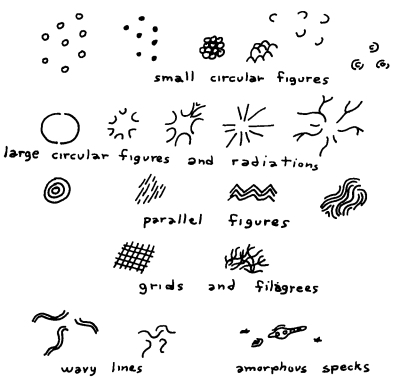
\includegraphics[width=0.4\textwidth]{../../Figures/hallucinations-visual.jpg} 
    \caption{Visualizations of hallucinations in schizophrenia \cite{Horowitz1964}.} 
    \label{fig:visualizations_hallucinations} 
\end{figure}


The overall structure is designed to simulate both subtle and intense hallucinatory experiences. Initial symptoms—such as whispers and the darkening of the visual field—represent the early stages of changes. As the simulation progresses, the intensity of both auditory and visual elements increases to reflect the overwhelming nature of more severe psychotic episodes. This progression helps users understand how hallucinations can escalate over time and provides insight into the lived experience of individuals with schizophrenia.

\section{Simulation Sequence}

To support this progression, Figure~\ref{fig:simulation_sequence} outlines the sequence and timing of both auditory and visual elements in the simulation. The structure is carefully chosen to reflect how psychotic symptoms often unfold—starting subtly and becoming more disruptive. Beginning with sort of a 'tunnel vision', by darkening the visual field and including whispered voices, the simulation gradually introduces more intense auditory cues and layered visual distortions, such as black stains and interactive colored dots. This stepwise increase in complexity ensures that users are not overwhelmed by the intensity of the symptoms. The timing is designed to fit within the short duration of the simulation (3 to 4 minutes), while still providing a productive experience of what psychosis might feel like. It should also be mentioned that the voice groups shown in Figure \ref{fig:simulation_sequence} are explained in more detail in the next chapter, where the implementation of the simulation is described.

\begin{figure}[p]
\centering
\begin{tikzpicture}[scale=0.72, transform shape,
  node distance=1.2cm and 2.2cm,
  roundnode/.style={circle, draw=black, fill=black!90, text=white, minimum size=1.2cm},
  purplenode/.style={ellipse, draw=black, fill=purple!20, minimum height=1cm, minimum width=1.6cm, align=center},
  yellownode/.style={rectangle, draw=black, fill=yellow!80, rounded corners, align=center, text width=2.8cm, font=\footnotesize},
  greynode/.style={rectangle, draw=black, fill=gray!20, rounded corners, align=center, text width=2.6cm, font=\footnotesize},
  every node/.style={font=\small}
]

% Central node
\node[roundnode] (startingpoint) {Start};

% Time checkpoints (reduced)
\node[purplenode, below=of startingpoint] (checkp01) {60 s};
\node[purplenode, below=of checkp01] (checkp03) {65 s};
\node[purplenode, below=of checkp03] (checkp06) {120 s};
\node[purplenode, below=of checkp06] (checkp08) {125 s};
\node[purplenode, below=of checkp08] (checkp11) {150 s};
\node[purplenode, below=of checkp11] (checkp12) {170 s};
\node[purplenode, below=of checkp12] (checkp14) {180 s};
\node[purplenode, below=of checkp14] (checkp15) {210 s};

% Connections (adjusted to preserve flow)
\draw (startingpoint) -- (checkp01);
\draw (checkp01) -- (checkp03);
\draw (checkp03) -- (checkp06);
\draw (checkp06) -- (checkp08);
\draw (checkp08) -- (checkp11);
\draw (checkp11) -- (checkp12);
\draw (checkp12) -- (checkp14);
\draw (checkp14) -- (checkp15);

% Annotations
\node[yellownode, right=of checkp01] (screendarkening) {Screen darkens};
\node[yellownode, right=of checkp06] (darkstains) {Black stains appear randomly every 2 s};
\node[yellownode, right=of checkp11] (darkstainsdisappear) {Stains disappear one by one};
\node[yellownode, right=of checkp12] (dots) {Dots appear — turn color when touched; repeat sound otherwise};
\node[yellownode, right=of checkp15] (dotsvansih) {Dots disappear};

\node[greynode, left=of checkp03] (voicegroup1to4) {Voice Groups 1–4};
\node[greynode, left=of checkp08] (voicegroup5to7) {Voice Groups 5–7};
\node[greynode, left=of checkp14] (voicegroup8to12) {Voice Groups 8–12};
\node[greynode, left=of checkp01] (whispers) {Whispers};

% Annotation connections
\draw (checkp01) -- (screendarkening);
\draw (checkp06) -- (darkstains);
\draw (checkp11) -- (darkstainsdisappear);
\draw (checkp12) -- (dots);
\draw (checkp15) -- (dotsvansih);
\draw (checkp01) -- (whispers);
\draw (checkp03) -- (voicegroup1to4);
\draw (checkp08) -- (voicegroup5to7);
\draw (checkp14) -- (voicegroup8to12);


\end{tikzpicture}
\caption{Sequence of time-structured voice and visual elements}
\label{fig:simulation_sequence}
\end{figure}
